\section{Classification}

To attempt classification, one method is to use linear regression and map all predictions greater than 0.5 as a 1 and all less than 0.5 as a 0. However, this method doesn't work well because classification is not actually a linear function.\\

The classification problem is just like the regression problem, except that the values we now want to predict take on only a small number of discrete values. For now, we will focus on the binary classification problem in which y can take on only two values, 0 and 1. (Most of what we say here will also generalize to the multiple-class case.) For instance, if we are trying to build a spam classifier for email, then $x^{(i)}$  may be some features of a piece of email, and y may be 1 if it is a piece of spam mail, and 0 otherwise. Hence, $y \in {0,1}$. 0 is also called the negative class, and 1 the positive class, and they are sometimes also denoted by the symbols “-” and “+.” Given $x^{(i)}$ the corresponding $y^{(i)}$ is also called the label for the training example.\\

Classification problems:\\
Email: Spam/Not Spam\\
Online Transaction: Valid/Fraud\\
Tumor: Malignant/Benign\\
$y \in {0,1}$ where 0 is the negative class and 1 is the positive class.\\

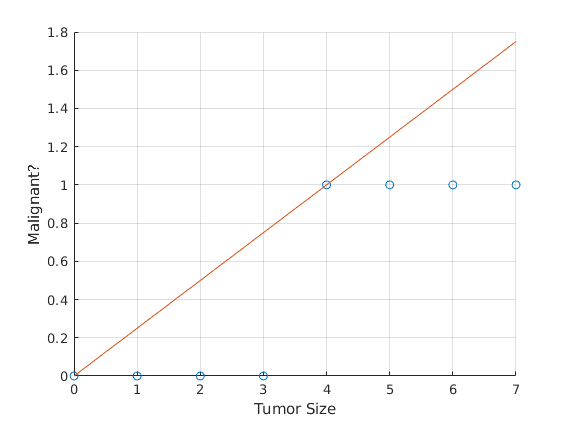
\includegraphics{matlab/classification.png}
For a few points that split up like this easily, the linear fit is not good.\\

Threshold Classifier output $h_{\theta}(x)$ at 0.5\\
if $h_{\theta}(x) \geq$ 0.5 y=1\\
if $h_{\theta}(x) <$ 0.5 y= 0\\
This is not perfect, still can mis-classify somethings.  It might be a reasonable solution. An outlier can skew the line.  This can move the thresold to the wrong location.  Linear regression is not a great idea for classification.

Logistic Regression outputs are always between 0 and 1.  The name includes regression but it is a classification algorithm\\
$$
0 \leq h_{\theta}(x) \leq 1
$$

\subsubsection{Hypothesis Representation}

We could approach the classification problem ignoring the fact that y is discrete-valued, and use our old linear regression algorithm to try to predict y given x. However, it is easy to construct examples where this method performs very poorly. Intuitively, it also doesn’t make sense for $h_\theta (x)$ to take values larger than 1 or smaller than 0 when we know that $y \in {0, 1}$. To fix this, let’s change the form for our hypotheses $h_\theta (x)$ satisfy $0 \leq h_\theta (x) \leq 1$. This is accomplished by plugging $\theta^Tx$ into the Logistic Function.


Our new form uses the "Sigmoid Function," also called the "Logistic Function":
\begin{equation}
  \begin{aligned}
    h_{\theta}(x) &= g(\theta^{T}x)\\
    z &= \theta^{T}x \\
    g(z) &= \frac{1}{1+e^{-z}}\\
    h_{\theta}(x) &= \frac{1}{1+e^{-\theta^{T}x}}
  \end{aligned}
\end{equation}

$g(z)$ is the Sigmoid or Logistic Function.  This is where the name Logistic Regression comes from.\\

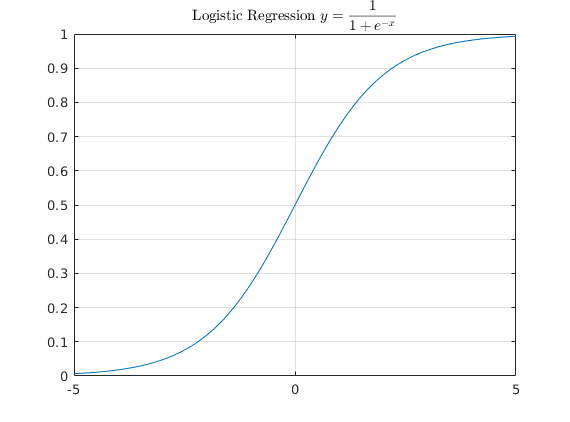
\includegraphics{matlab/logistic_plot.png}

The function g(z), shown here, maps any real number to the (0, 1) interval, making it useful for transforming an arbitrary-valued function into a function better suited for classification.\\


$h_{\theta}(x)$ will give us the probability that our output is 1. For example, $h_\theta(x)=0.7$ gives us a probability of 70\% that our output is 1. Our probability that our prediction is 0 is just the complement of our probability that it is 1 (e.g. if probability that it is 1 is 70\%, then the probability that it is 0 is 30\\

\begin{equation}
  \begin{aligned}
  &h_\theta(x) = P(y=1 \| x ; \theta) &= 1 - P(y=0 | x ; \theta) \\
  &P(y = 0 \| x;\theta) + P(y = 1 | x ; \theta) = 1
  \end{aligned}
\end{equation}

Fit parameters $\theta$ to our data.\\
$h_{\theta}(x)$ = estimate probability that y=1 on input x\\


Example:\\
$
x =
\begin{bmatrix}
  x_{0} \\
  x_{1} \\
\end{bmatrix}
$ =
$
\begin{bmatrix}
  1 \\
  tumor size \\
\end{bmatrix}
$\\

If $h_{\theta}(x)$ = 0.7, then it is a 70\% chance of being a tumor.


\subsubsection{Decision Boundary}

In order to get our discrete 0 or 1 classification, we can translate the output of the hypothesis function as follows:
\begin{equation}
  \begin{aligned}
    & h_\theta(x) \geq 0.5 \rightarrow y = 1 \\
    & h_\theta(x) < 0.5 \rightarrow y = 0 \\
  \end{aligned}
\end{equation}

The way our logistic function g behaves is that when its input is greater than or equal to zero, its output is greater than or equal to 0.5:

\begin{equation}
  \begin{aligned}& g(z) \geq 0.5 \\
    & when \; z \geq 0\end{aligned}
\end{equation}

Remember.

\begin{equation}
  \begin{aligned}
    z=0, e^{0}=1 \Rightarrow g(z)=1/2\\
    z \to \infty, e^{-\infty} \to 0 \Rightarrow g(z)=1\\
    z \to -\infty, e^{\infty}\to \infty \Rightarrow g(z)=0
  \end{aligned}
\end{equation}

So if our input to g is $\theta^{T}X$ then that means:
\begin{equation}
  \begin{aligned}
    & h_\theta(x) = g(\theta^T x) \geq 0.5 \\
    & when \; \theta^T x \geq 0
  \end{aligned}
\end{equation}

From these statements we can now say:
\begin{equation}
  \begin{aligned}
    & \theta^T x \geq 0 \Rightarrow y = 1\\
    & \theta^T x < 0 \Rightarrow y = 0 \\
  \end{aligned}
\end{equation}

The \textbf{decision boundary} is the line that separates the area where y = 0 and where y = 1. It is created by our hypothesis function.

Example:
\begin{equation}
  \begin{aligned}
    & \theta = \begin{bmatrix}
      5\\
      -1\\
      0\\
    \end{bmatrix}\\
     & y = 1 \; if \; 5 + (-1) x_1 + 0 x_2 \geq 0\\
     & 5 - x_1 \geq 0\\
     & - x_1 \geq -5\\
    & x_1 \leq 5\\
     \end{aligned}
\end{equation}

In this case, our decision boundary is a straight vertical line placed on the graph where $x_1$ =5, and everything to the left of that denotes y = 1, while everything to the right denotes y = 0.\\

Again, the input to the sigmoid function g(z) (e.g. $\theta^T X$ doesn't need to be linear, and could be a function that describes a circle (e.g. z = $\theta_0 + \theta_1 x_1^2 +\theta_2 x_2^2$ or any shape to fit our data.

Example:\\
If $h_{\theta}(x) = g(\theta_{0} + \theta_{1}x_{1} + \theta_{2}x_{2})$ then predict y =1.\\
For given $ \theta = \begin{bmatrix}
  -3\\
  1\\
  1\\
\end{bmatrix}$\\
then $ -3 + x_{1} + x_{2} \geq 0 $.\\
This means $\theta^{T}x = -3 + x_{1} + x_{2} + \theta_{3}x_{1}^{2} + \theta_{4}x_{2}^{2})$\\

\textbf{Non-Linear Decision Boundaries}
$h_{\theta}(x) = g(\theta_{0} + \theta_{1}x_{1} + \theta_{2}x_{2}$\\
$
\begin{aligned}
  & \theta = \begin{bmatrix}
    -1\\
    0\\
    0\\
    1\\
    1\\
  \end{bmatrix}
\end{aligned}\\
$\\
This will predict y =1 if $-1 + x_{1}^{2} + x_{2}^{2} \geq 0$

Decision Boundary is property not of training set but of the hypothesis and parameters. \\

You can use even higher order polynomials leading to very complex decision boundaries.

\subsection{Logistic Regression Model}
\subsubsection{Cost Function}
\subsubsection{Simplified Cost Function and Gradient Descent}
\subsubsection{Advanced Optimization}

\subsection{Multiclass Classification}
\subsubsection{One Vs All}

\subsection{Overfitting}
\subsubsection{Cost Function}
\subsubsection{Regularized Linear Regression}
\subsubsection{Regularized Logistic Regression}


